\documentclass{article}
\usepackage[utf8]{inputenc}
\usepackage{amsmath,amsfonts,amssymb} % Paquetes para matemáticas
\usepackage{ulem} % Para subrayar texto
\usepackage{geometry}
\usepackage{indentfirst}
\usepackage{graphicx}
\usepackage{float}
\usepackage[backend=biber,style=apa]{biblatex}
\addbibresource{bibliografia.bib}
\usepackage{subcaption}


\geometry{
    a4paper,
    left=2cm,
    right=2cm,
    top=2.5cm,
    bottom=2.5cm,
    includefoot,
    headheight=15pt,
    headsep=0.5cm,
    footskip=1cm
}

\title{TP2 - Sistema de predicción de skips en Spotify}
\author{Dafydd Jenkins, Josefina Jahde, Serena Marelli}
\date{\today}

\begin{document}

\maketitle

\section*{Introducción}

En el presente trabajo se aborda el desarrollo de un sistema de predicción de \textit{skips} en Spotify, es decir, la acción de un usuario de saltear una canción antes de que termine. Este fenómeno es de alto interés para plataformas de streaming, ya que constituye una señal directa del desinterés del usuario hacia un contenido, y puede ser aprovechado tanto para mejorar sistemas de recomendación como para comprender mejor los hábitos de escucha.

El objetivo principal fue construir un modelo que, a partir de información disponible en los eventos de reproducción (como el momento del día, el dispositivo utilizado o la razón de inicio de la canción), logre anticipar si una canción será o no salteada por el usuario. Para esto, se trabajó con un conjunto de datos provisto por la cátedra, compuesto por millones de eventos de reproducción anónimos a lo largo de una década.

El desafío no solo radicó en lograr un buen desempeño predictivo, sino también en evitar problemas comunes en series temporales, como el \textit{data leakage}, y en seleccionar correctamente las variables más relevantes para el modelo. Se exploraron distintas estrategias de validación y diversos algoritmos de aprendizaje automático, incluyendo regresión logística, Random Forest y XGBoost, junto con una ingeniería de atributos específica que buscó capturar patrones de comportamiento del usuario.

La implementación del modelo se encuentra dividida en dos archivos, \texttt{funciones.py} y \texttt{implementacion.ipynb}, ambos subidos junto con este informe. En el primero se encuentran implementados todos las funciones necesarias para el procesamiento de datos. En el segundo, se encuentran el código usado para:

\begin{itemize}
	\item Análisis exploratorio de datos
	\item Procesamiento de datos (\textit{feature engineering})
	\item Validación de modelos
	\item Búsqueda de hiperparámetros
	\item Creación de los modelos usados durante la realización del trabajo
	\item Modelo final y exportación de predicciones
	\item Evaluación de importancia de atributos del modelo final
\end{itemize}

\section*{Análisis exploratorio de datos}
Para comenzar, se realizó un análisis exploratorio de los datos dados. Esto incluye tipos de atributos, valores faltantes, proporciones de clases y media, std y cuartiles para las variables numéricas.

Luego, con el objetivo de entender el comportamiento de la variable \texttt{TARGET} (indicadora de si un usuario “saltea” una canción) en relación con atributos temporales del evento de reproducción, graficamos la cantidad de skips por hora, dia de semana, mes y año.

\begin{figure}[H]
    \centering
    \begin{subfigure}[b]{0.45\textwidth}
        \centering
        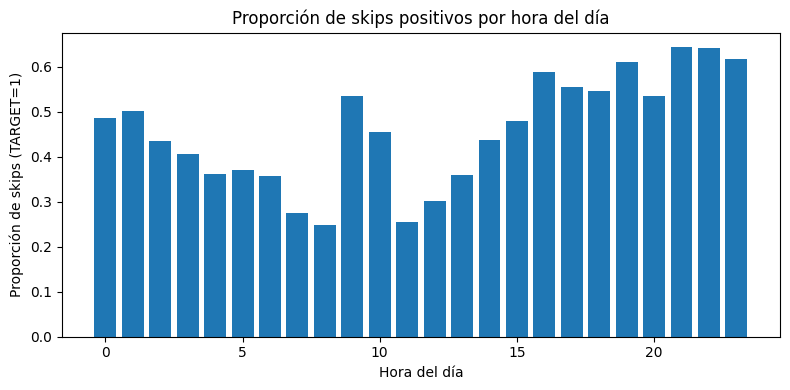
\includegraphics[width=\textwidth]{figuras/hora.png}
        \caption{Proporción de skips por hora}
    \end{subfigure}
    \begin{subfigure}[b]{0.45\textwidth}
        \centering
        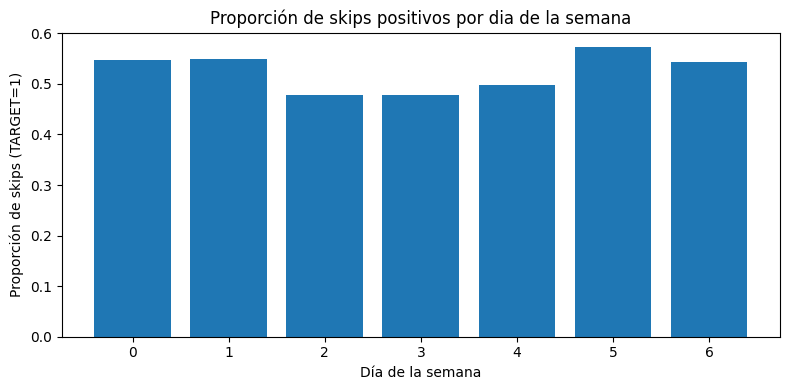
\includegraphics[width=\textwidth]{figuras/dia.png}
        \caption{Proporción de skips por día de la semana}
    \end{subfigure}

    \vspace{0.5cm}

    \begin{subfigure}[b]{0.45\textwidth}
        \centering
        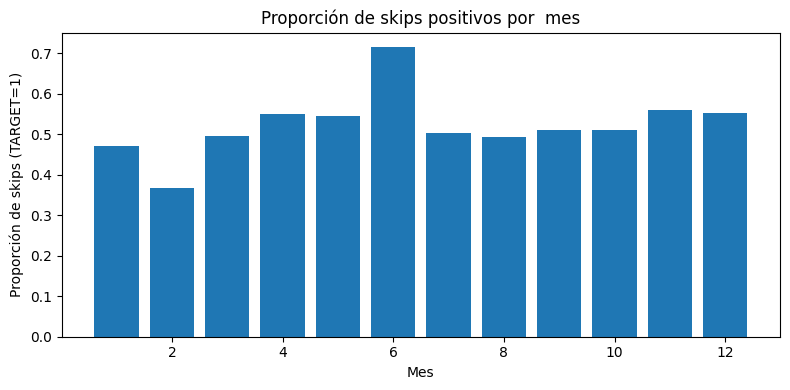
\includegraphics[width=\textwidth]{figuras/mes.png}
        \caption{Proporción de skips por mes}
    \end{subfigure}
    \begin{subfigure}[b]{0.45\textwidth}
        \centering
        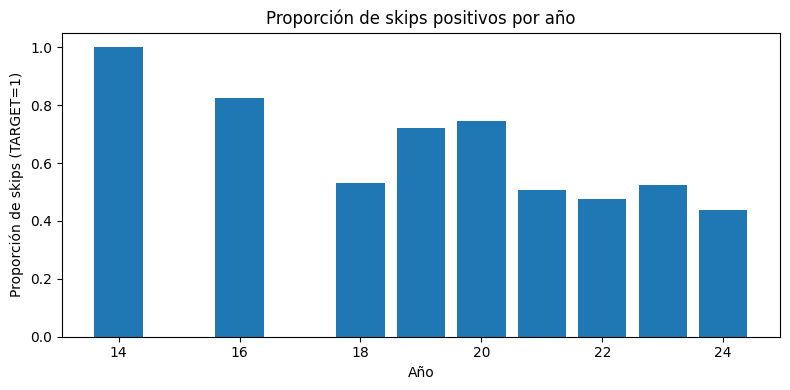
\includegraphics[width=\textwidth]{figuras/año.png}
        \caption{Proporción de skips por año}
    \end{subfigure}
    
    \caption{Distribución temporal de la variable objetivo}
    \label{fig:temporal_target_distribution}
\end{figure}

Para el día de la semana se observó una distribución heterogénea, con algunos días (por ejemplo, los lunes y viernes) registrando mayor cantidad de skips, lo cual podría vincularse con patrones de comportamiento semanales de los usuarios, como escuchar música mientras trabajan o durante traslados.

En la visualización de la hora del día se observa un incremento claro de actividad y de skips durante ciertos tramos horarios (por ejemplo, en horas laborales o de la tarde), lo que sugiere una fuerte componente temporal en el comportamiento del usuario que podría ser aprovechado por el modelo.

Para el mes, se ve que no hay un patrón claro que pueda indicar un cierto comportamiento en el salteo de canciones.

Para el año, se ven cosas extrañas, como que en 2015 y 2017 no se registran skips. Además, pareciera que la proporción de skips baja, en lineas generales, con el pasar de los años. Esto podría deberse, por ejemplo, a mejoras en el sistema de recomendación de canciones de Spotify a lo largo del tiempo.

\subsection*{Correlación entre variables}
Para entender mejor la correlación entre las variables, se generó una matriz de correlación. Esta nos permite  estudiar las relaciones lineales entre las variables numéricas del dataset e identificar atributos redundantes, relaciones inesperadas o dependencias que podrían ser aprovechadas.

\begin{figure}[H]
	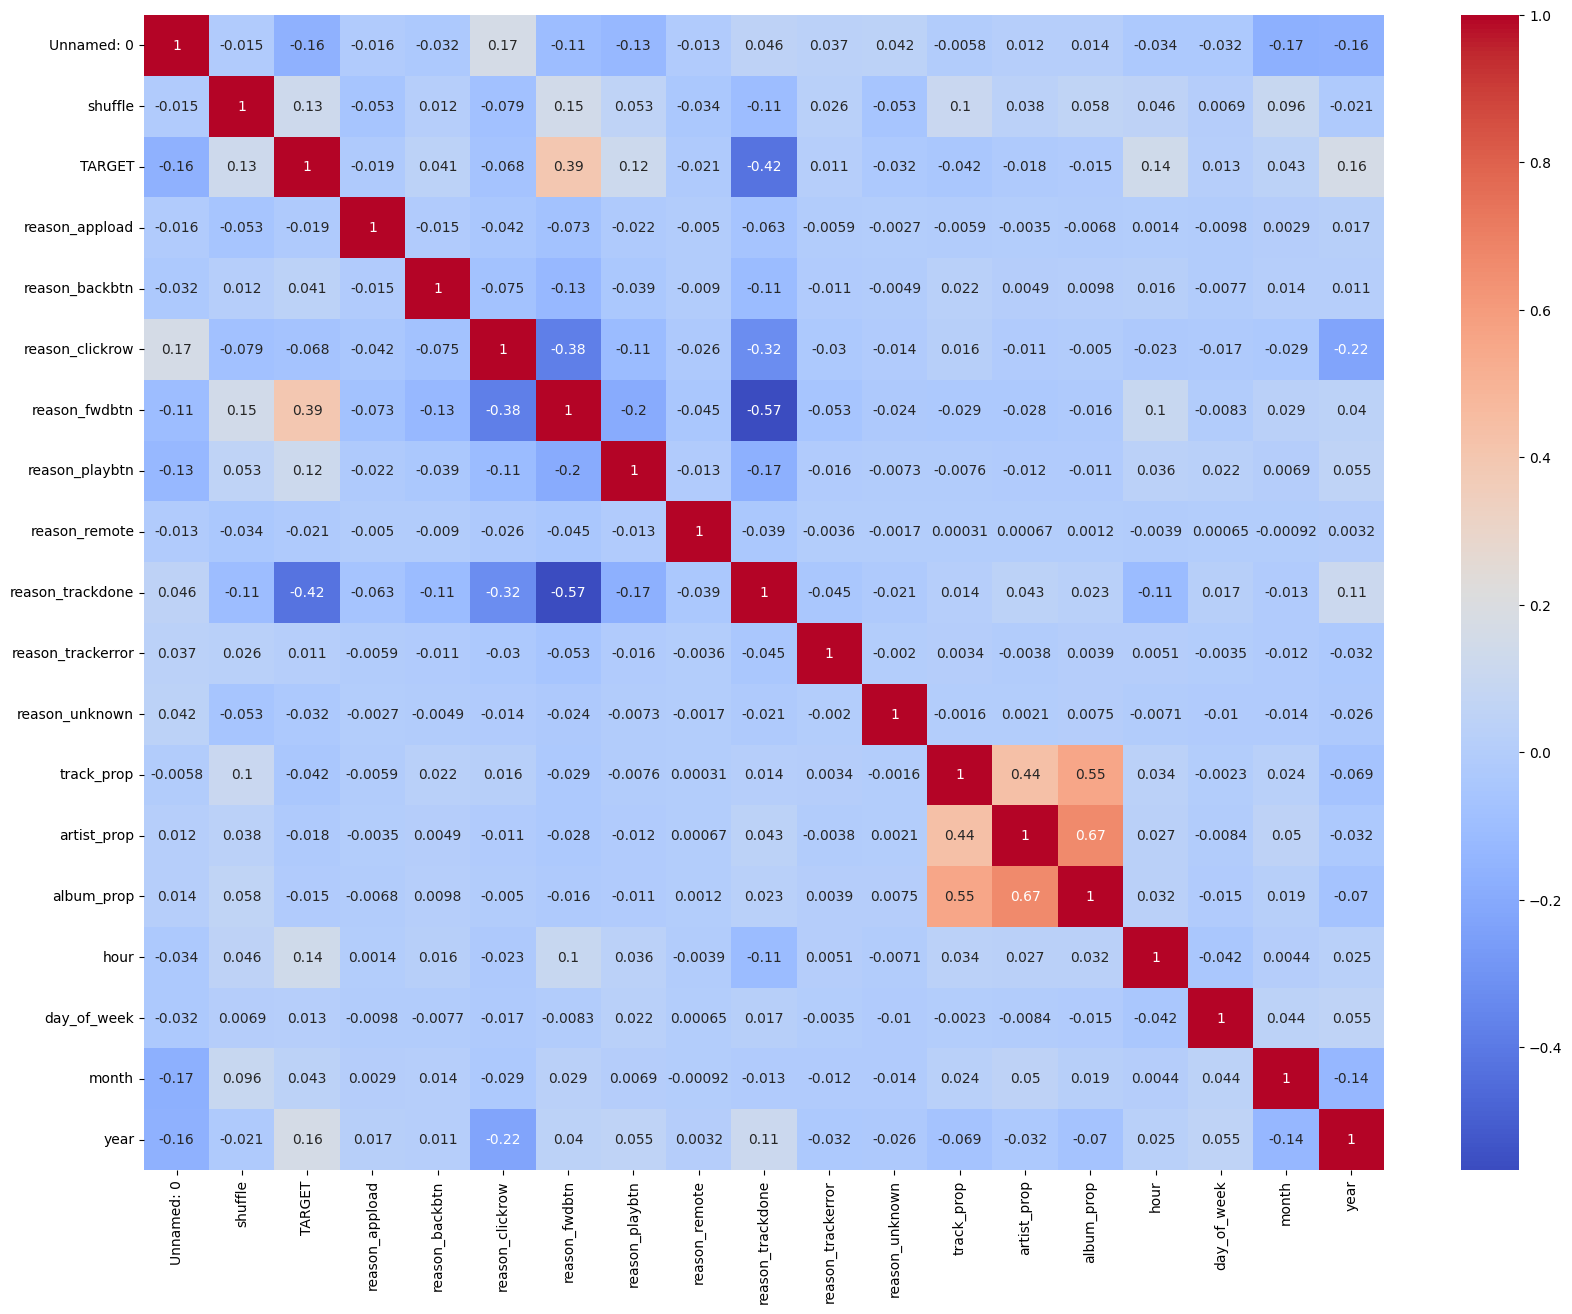
\includegraphics[width=\textwidth]{figuras/matriz_corr.png}
	\caption{Matriz de correlación entre atributos}
    	\label{fig:matriz_corr}
\end{figure}

Entre los resultados más relevantes del análisis, se destacan:

\begin{itemize}
	\item Alta correlación entre \texttt{track\_prop}, \texttt{artist\_prop} y \texttt{album\_prop}: estas variables representan la proporción histórica de skips para cada canción, artista o álbum. El hecho de que estén fuertemente correlacionadas sugiere que en muchos casos el comportamiento del usuario frente a una canción está fuertemente condicionado por el artista o álbum, lo que puede indicar redundancia o multicolinealidad entre ellas.
	\item Relaciones moderadas entre variables temporales derivadas: variables como\texttt{hour}, \texttt{day\_of\_week} o \texttt{month} no presentan correlaciones lineales fuertes entre sí ni con la variable objetivo, pero igualmente pueden ser útiles en interacciones no lineales (como las que capta un modelo como \texttt{XGBoost}).
	\item \texttt{duration\_ms} tiene muy baja correlación con el resto: esto indica que la duración de la canción podría ser una señal útil independiente, aunque por sí sola no predice el skip.
	\item Hay una correlación entre \texttt{TARGET} y \texttt{reason\_fwdbtn} igual a 0.39, la cual es la más alta entre las razones de reproducción, indicando que cuando la razón de inicio es fwdbtn, hay más probabilidad de que \texttt{TARGET} sea 1 (el usuario escuche la canción entera o al menos más de una fracción mínima). 
	\item Podemos observar también que\texttt{reason\_trackdone} correlaciona negativamente con \texttt{TARGET} (-0.42), es la más baja entre las razones. 

\end{itemize}

En base a los dos últimos puntos, decidimos analizar el \texttt{TARGET} con respecto a todas las razones de inicio.

\begin{figure}[H]
    \centering
    \begin{subfigure}[b]{0.45\textwidth}
        \centering
        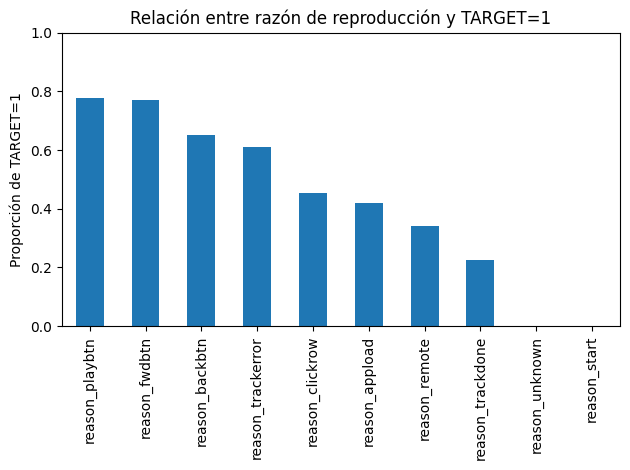
\includegraphics[width=\textwidth]{figuras/reasons_target1.png}
    \end{subfigure}
    \begin{subfigure}[b]{0.45\textwidth}
        \centering
        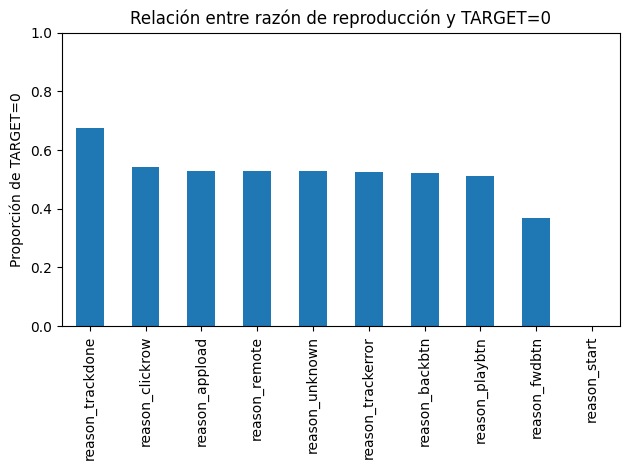
\includegraphics[width=\textwidth]{figuras/reasons_target0.png}
    \end{subfigure}
\end{figure}

Para la proporción de \texttt{TARGET}=1 según razón de inicio, vemos que:

\begin{itemize}
	\item las variables \texttt{reason\_playbtn} y \texttt{reason\_fwdbtn} presentan las proporciones más altas (cercanas a 0.8), lo que indica que cuando el usuario inicia la reproducción de forma manual (ya sea presionando play o adelantando), hay un mayor nivel de compromiso o interés. Les siguen \texttt{reason\_backbtn} y \texttt{reason\_trackererror}, con valores por encima de 0.6, lo cual también refleja una cierta intención de interacción voluntaria por parte del usuario.
	\item En contraste, variables como \texttt{reason\_clickrow}, \texttt{reason\_appload}, \texttt{reason\_trackdone}, \texttt{reason\_remote} y \texttt{reason\_unknown} muestran proporciones menores a 0.5. Esto sugiere que estas formas de inicio —muchas veces automáticas o sin acción directa del usuario— están asociadas con un menor nivel de compromiso y, por ende, una menor probabilidad de alcanzar el TARGET=1.
\end{itemize}

También se construyó un gráfico que muestra la proporción de eventos con \texttt{TARGET} = 0 (es decir, canciones que no fueron salteadas) para cada una de las categorías de \texttt{reason\_start}.
Los hallazgos principales son:


\begin{itemize}
	\item La categoría trackdone tiene una proporción alta de \texttt{TARGET} = 0. Esto es esperable: esta razón indica que la canción comenzó automáticamente al terminar la anterior, lo que en general implica que el usuario está dejando correr la música sin intervenir, y por ende, es menos probable que saltee.
	\item Las razones clickrow, fwdbtn y backbtn muestran menores proporciones de no-skip. Estas razones implican una acción explícita del usuario, muchas veces asociada a una búsqueda activa o a navegación, por lo que es más probable que ocurran skips.
	\item appload y remote también presentan proporciones altas de no-skips, lo cual podría deberse a que reflejan inicios más pasivos (por ejemplo, cuando la app inicia o cuando la música se lanza desde un dispositivo externo).
\end{itemize}

Este análisis parece indicar que \texttt{reason\_start} es una variable muy informativa respecto del comportamiento del usuario, y justifica su inclusión en el modelo.

\section*{Variables creadas}

A partir del atributo \texttt{ts} (timestamp), creamos los atributos \texttt{hour}, \texttt{day\_of\_week}, \texttt{month} y \texttt{year}, que indican la hora, día de la semana (donde 0 es lunes y 6 es domingo), mes y año en que finalizó la reproducción.

Creamos una variable binaria \texttt{is\_iphone}, que indica si la reproducción se dio en un iPhone. Esta variable se construyó a partir del atributo \texttt{platform}, bajo la hipótesis de que es más común saltear una canción desde el teléfono móvil. Notamos que no había registros de teléfonos Android u otros dispositivos móviles distintos de iPhone.

Obtuvimos la variable \texttt{duration\_ms} (duración de la canción en milisegundos) a partir del URI del track, consultando la API de Spotify.

La variable \texttt{is\_early\_finish} determina si una reproducción finalizó antes de lo esperado, es decir, si no llegó a reproducirse la canción completa. Esta variable se calcula a partir de \texttt{ts} y \texttt{duration\_ms}. En términos generales, si la diferencia entre el timestamp actual y el anterior es menor a la duración de la canción menos 2 segundos, se considera que la canción terminó prematuramente. Si esa diferencia es menor a 9 minutos (percentil 95 de la duración de todas las canciones), se considera que las reproducciones están pegadas temporalmente, por lo que no se marca como terminación prematura. Finalmente, si la diferencia entre timestamps es mayor a 9 minutos, se considera que hubo un bache entre escuchas, y no se puede determinar si la canción terminó prematuramente o no.

El atributo \texttt{racha\_skips\_prev} se calcula a partir del \texttt{TARGET} de las observaciones anteriores. Si la observación anterior fue un skip, \texttt{racha\_skips\_prev} será igual al de la observación anterior incrementado en uno. Si no fue skip, se reinicia a 0. Si no se tiene el dato del \texttt{TARGET} anterior (por ejemplo, en \texttt{submission.csv}), se hereda el valor de la observación anterior. Para generar esta variable en el conjunto de \texttt{submission}, se unieron momentáneamente los datos de \texttt{submission} y \texttt{competition\_data}, se ordenaron cronológicamente, se calculó la racha, y se extrajo la columna final para usarla en predicción.

Aplicamos \textit{one-hot encoding} a la variable categórica \texttt{reason\_start}, obteniendo las variables \texttt{reason\_appload}, \texttt{reason\_backbtn}, \texttt{reason\_clickrow}, \texttt{reason\_fwdbtn}, \texttt{reason\_playbtn}, \texttt{reason\_remote} y \texttt{reason\_trackdone}.

Las variables \texttt{track\_prop}, \texttt{artist\_prop} y \texttt{album\_prop} se crearon a partir de \texttt{master\_metadata\_track\_name}, \texttt{master\_metadata\_album\_artist\_name} y \texttt{master\_metadata\_album\_album\_name}, respectivamente. Representan la proporción de skips para cada track, artista o álbum, y se calculan mediante conteo de eventos históricos.

La variable \texttt{hour\_day\_of\_week} se obtuvo como combinación polinómica de \texttt{hour} y \texttt{day\_of\_week}. Se probaron varias combinaciones, y esta fue la única que aportó valor al modelo.

Adicionalmente, se obtuvo el género musical de cada artista, agrupado en 6 categorías: \textit{Pop/Rock}, \textit{Urban}, \textit{Electronica}, \textit{Regional}, \textit{Otros} y \textit{Unknown}. Para lograr esto, se utilizó la API de Spotify para obtener el ID del artista a partir del URI del track, y luego se consultaron los géneros asociados. Con ayuda de ChatGPT se agruparon las respuestas en las 6 macro-categorías. El proceso está documentado en el siguiente enlace: \texttt{https://chatgpt.com/share/68198985-5d44-800c-801c-42031350eeb0}.

Sin embargo, mediante validación se observó que esta variable no mejoraba el rendimiento del modelo y contribuía al sobreajuste (mejor desempeño en entrenamiento, pero peor en validación). Por esta razón, fue descartada en la versión final del modelo.

\section*{Estrategias de validación}

Utilizamos tres formas distintas de validar nuestros modelos.

La primera fue un \textbf{holdout set temporal}, en el cual se entrenaba el modelo con el primer 70\% de los datos ordenados cronológicamente, y se predecía sobre el 30\% restante. Esta división se realizó con el objetivo de evitar \textit{data leakage} entre entrenamiento y validación, asegurando que nunca se entrenara con eventos posteriores a aquellos que se buscaba predecir. Sin embargo, observamos que la estimación del AUC obtenida con esta estrategia era muy distinta de la que reportaba Kaggle al hacer el \textit{submmit}, y estaba fuertemente influenciada por el período temporal de los datos seleccionados.

Por este motivo, pasamos a utilizar el método \textbf{Time Series Cross Validation} que ofrece \texttt{Scikit-learn}. Esta estrategia también respeta la temporalidad (es decir, cada \textit{fold} entrena con datos previos a los del conjunto de validación) y producía estimaciones del AUC algo más cercanas a las reales. Sin embargo, aún persistía una diferencia importante entre la performance en validación y la performance observada en Kaggle. Observamos que muchos cambios que mejoraban la métrica en validación terminaban empeorando los resultados finales del \textit{submit}.

Nuestra hipótesis es que esta discrepancia se debía a que, en el entorno real de predicción (cuando generamos el archivo de \texttt{submission.csv}), el modelo era entrenado con datos de todos los años y debía predecir también sobre datos distribuidos en todos los años. Esto significa que, por ejemplo, el modelo debía predecir observaciones del año 2016 habiendo sido entrenado con información del 2024 y viceversa, una situación que ninguna de las validaciones anteriores lograba replicar.

Por este motivo, implementamos una tercera forma de validación que llamamos \textbf{holdout aleatorio}. Esta consistía en seleccionar aleatoriamente el 30\% de los datos de entrenamiento como conjunto de validación. Esta proporción fue elegida porque \texttt{submission.csv} representaba aproximadamente un 30\% del total de observaciones, y además, las observaciones parecían haber sido seleccionadas de forma aleatoria. 

Una vez hecha esta partición, se replicaba exactamente el mismo procedimiento que se utilizaba para hacer el \textit{submit}: se ocultaba temporalmente la variable \texttt{TARGET} en \texttt{validation} (para evitar \textit{leakage} durante el cálculo de variables), se unían \texttt{train} y \texttt{validation} para calcular las columnas \texttt{is\_early\_finish} y \texttt{racha\_skips\_prev}, y luego estas se reintegraban en \texttt{validation}. Finalmente, se entrenaba el modelo con \texttt{train} y se predecía sobre \texttt{validation}, recuperando la variable \texttt{TARGET} original para calcular el AUC.

Reconocemos que esta estrategia tiene una alta probabilidad de introducir \textit{data leakage}, y que desde el punto de vista teórico es la menos rigurosa. Sin embargo, en la práctica fue la que mejor reflejó la performance que luego obteníamos en Kaggle, y por ello fue la que utilizamos para la evaluación final y comparación entre modelos.

\section*{Modelos predictivos utilizados}

Comenzamos utilizando un modelo de \textbf{regresión logística}, que fue el empleado para realizar el primer \textit{submit}. Este modelo alcanzó un AUC en Kaggle de apenas 0.56, por lo que fue rápidamente descartado, aun cuando no contábamos en ese momento con todos los atributos que luego formarían parte del modelo final.

Luego pasamos a utilizar un \textbf{Random Forest}. Este modelo mejoró significativamente la performance respecto a la regresión logística, sin requerir una gran cantidad de atributos adicionales. En esta instancia, solo incorporamos el \textit{one-hot encoding} de la variable \texttt{reason\_start}, la duración de la canción (\texttt{duration\_ms}) y las proporciones de aparición de cada track, artista y álbum. Con esta configuración, logramos alcanzar un AUC de 0.89 en Kaggle, incluso sin realizar aún búsqueda de hiperparámetros.

Posteriormente, probamos con \textbf{XGBoost}, utilizando exactamente los mismos atributos e igualmente sin ajuste de hiperparámetros. Este modelo superó al anterior alcanzando un AUC de 0.91, lo que nos llevó a adoptarlo como modelo final. Fue sobre este modelo que realizamos una búsqueda más exhaustiva de hiperparámetros, además de aplicar ingeniería de atributos adicional.

Para la búsqueda de hiperparámetros, realizamos un \textbf{grid search} sobre los parámetros \texttt{reg\_lambda}, \texttt{gamma} y \texttt{learning\_rate}, utilizando como estrategia de validación el \textit{holdout set aleatorio}, repetido sobre cinco semillas distintas. Elegimos esta forma de validación para reducir la varianza entre los AUCs estimados y obtener un resultado representativo del comportamiento del modelo al momento del \textit{submit}.

Los mejores hiperparámetros obtenidos fueron: \texttt{reg\_lambda = 5}, \texttt{gamma = 0} y \texttt{learning\_rate = 0.3}. Cabe destacar que cada vez que modificábamos el conjunto de atributos utilizados en el modelo, volvíamos a ejecutar la búsqueda de hiperparámetros para adaptarlos al nuevo espacio de variables.

\section*{Importancia de atributos}

Para evaluar qué atributos fueron más relevantes en la predicción del objetivo (\texttt{TARGET}), se utilizó la métrica \textit{Gain} proporcionada por XGBoost. Esta métrica mide la mejora esperada en la función objetivo (ganancia) cuando una feature es utilizada para realizar una división en un árbol del modelo.

\begin{figure}[H]
    \centering
    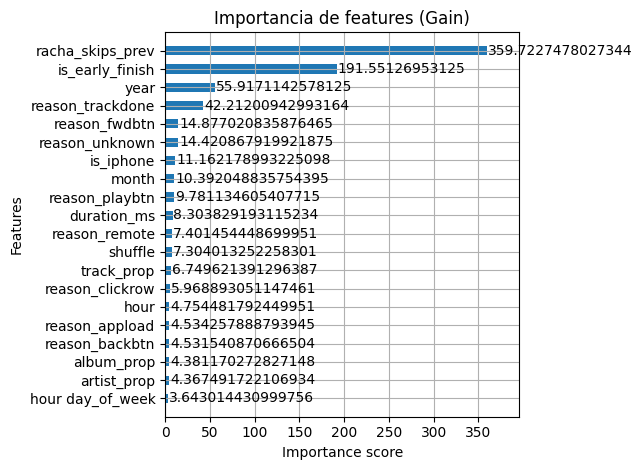
\includegraphics[width=0.85\textwidth]{figuras/gains.png}
    \caption{Importancia de atributos medida por Gain (XGBoost)}
    \label{fig:feature_importance}
\end{figure}

Como se observa en la Figura~\ref{fig:feature_importance}, los atributos más importantes fueron:

\begin{itemize}
    \item \texttt{racha\_skips\_prev}: con una ganancia significativamente superior al resto ($\approx$ 360), esta variable indica la cantidad de skips consecutivos previos al evento actual. Su alta importancia sugiere que el comportamiento reciente del usuario es un fuerte predictor de futuros skips, evidenciando patrones conductuales estables.
    
    \item \texttt{is\_early\_finish}: esta variable detecta si la canción anterior se terminó antes de lo esperado. Con una ganancia de aproximadamente 192, su alta relevancia indica que las interrupciones prematuras en una reproducción se asocian con una mayor probabilidad de que la siguiente canción también sea salteada.
    
    \item \texttt{year}: el año del evento aporta una ganancia moderada ($\approx$ 56), lo que sugiere la existencia de tendencias temporales en el comportamiento del usuario, posiblemente relacionadas con cambios en la plataforma, el algoritmo de recomendación o los hábitos de consumo musical.
\end{itemize}

Otros atributos con influencia media incluyen ciertas razones de reproducción (\texttt{reason\_trackdone}, \texttt{reason\_fwdbtn}, \texttt{reason\_unknown}), el tipo de dispositivo (\texttt{is\_iphone}) y variables temporales como \texttt{month}. Esto refuerza la idea de que tanto el contexto del evento como la forma en que se inició la reproducción inciden en la probabilidad de skip.

En contraste, variables como \texttt{album\_prop}, \texttt{artist\_prop} y \texttt{hour\_day\_of\_week} presentaron valores de ganancia muy bajos, lo cual sugiere que aportan poco valor predictivo frente a las variables de comportamiento directo.

En resumen, el modelo asigna mayor importancia a variables que capturan el \textbf{comportamiento reciente del usuario}, y en menor medida a características contextuales o del contenido. Este hallazgo valida el enfoque conductual adoptado durante la construcción del sistema.

\section*{Conclusiones y trabajo futuro}

A lo largo del trabajo, logramos construir un sistema predictivo robusto que permite anticipar con alta precisión si una canción será salteada. Mediante la incorporación de variables que capturan el comportamiento reciente del usuario (como \texttt{racha\_skips\_prev} e \texttt{is\_early\_finish}) y el uso del modelo XGBoost con hiperparámetros ajustados, alcanzamos una performance destacada en la plataforma de evaluación (AUC $\approx$ 0.97).

Uno de los principales aprendizajes fue la importancia de elegir correctamente los atributos predictores. La incorporación de los atributos \texttt{racha\_skips\_prev} e \texttt{is\_early\_finish} mejoró enormemente la performance del modelo, mucho más de lo que lo hizo la búsqueda de hiperparámtros, por ejemplo.

Además, vimos la importancia de elegir correctamente la estrategia de validación. Observamos que métodos tradicionales, incluso aquellos que respetan la temporalidad, no siempre reflejan con fidelidad el comportamiento real del modelo en producción. En cambio, una validación aleatoria que replicara mejor el entorno de testeo de Kaggle resultó más representativa.

Como posibles mejoras futuras, se identifican varias líneas de trabajo:
\begin{itemize}
    \item Incorporar información del contenido de las canciones (como género musical, BPM, energía, etc.) de forma más efectiva, evitando el sobreajuste observado en pruebas preliminares.
    \item Aplicar técnicas de \textit{embedding} para representar entidades categóricas de alta cardinalidad como canciones o artistas.
\end{itemize}

En definitiva, el sistema desarrollado demuestra que es posible predecir con alta precisión los skips de canciones utilizando únicamente información contextual y de comportamiento reciente, aportando así una herramienta potencialmente útil para sistemas de recomendación y análisis de usuarios en plataformas de música digital.

\end{document}